\subsection{\texttt{increasing\_loop}}
\label{subsec:increasing_loop}

\begin{flushright}
\textbf{Author} \\
Oliver Sheridan-Methven
\end{flushright}

The increasing loop algorithm is a stochastic algorithm which produces a possible solution for the travelling salesman problem, which will most likely not be optimal. However, the algorithm is constructed to hopefully provide near optimal solutions, and possibly some optimal, over a small set of runs, although it is not guaranteed. The hope is that this scheme is a reasonable compromise between execution time and optimality.

The algorithm begins by randomly selecting three vertices and forming a loop between them, containing only these three\footnote{We can assume that we have more than 3 vertices, else the solution is trivial.}. Then with this sub-loop, we consider an arbitrary vertex not contained in the sub-loop. For this unconnected vertex, we evaluate the added distance to the loop if we were to include this vertex and form a larger sub-loop. We compute which connection in the loop would need to be changed that would given the minimal distance increase. This involves evaluating the added distance from replacing each existing connection.
Noting what the increased distance would be, we repeat this for all the nodes not in the sub-loop, and hence find what the global minimal deformation to the loop would be if we had to include one of the unconnected points. We form this minimal connection, and then recompute what the next minimal global deformation would be. We perform this scheme iteratively until there are no unconnected vertices. A depiction of the scheme is shown in Figure~\ref{fig:increasing_loop}.


\begin{figure}[htb]
\centering
\begin{subfigure}{0.3\textwidth}
\centering
\fbox{\begin{tikzpicture}
\draw[fill] (0,0) circle (2pt) coordinate (a);
\draw[fill] (0.4,3) circle (2pt) coordinate (b);
\draw[fill] (2,3.4) circle (2pt) coordinate (c);
\draw[fill] (3.5,0.7) circle (2pt) coordinate (d);
\draw[fill] (1,1) circle (2pt) coordinate (e);
\draw[fill] (2,2) circle (2pt) coordinate (f);
\draw[fill] (3,0.7) circle (2pt) coordinate (g);
\end{tikzpicture}}
\caption{Initial configuration.}
\label{subfig:increasing_loop_step_0}
\end{subfigure}
\begin{subfigure}{0.3\textwidth}
\centering
\fbox{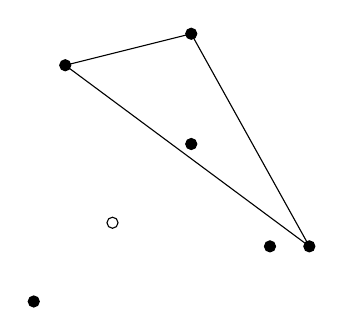
\begin{tikzpicture}
\draw[fill] (0,0) circle (2pt) coordinate (a);
\draw[fill] (0.4,3) circle (2pt) coordinate (b);
\draw[fill] (2,3.4) circle (2pt) coordinate (c);
\draw[fill] (3.5,0.7) circle (2pt) coordinate (d);
\draw[] (1,1) circle (2pt) coordinate (e);
\draw[fill] (2,2) circle (2pt) coordinate (f);
\draw[fill] (3,0.7) circle (2pt) coordinate (g);
\draw (b)--(d);
\draw (b)--(c);
\draw (c)--(d);
\end{tikzpicture}}
\caption{Initialisation.}
\label{subfig:increasing_loop_step_1}
\end{subfigure}
\begin{subfigure}{0.3\textwidth}
\centering
\fbox{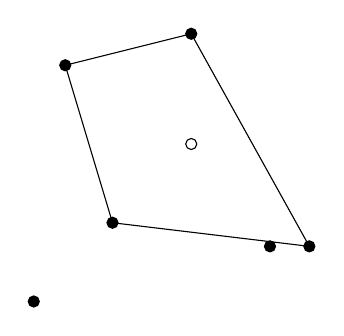
\begin{tikzpicture}
\draw[fill] (0,0) circle (2pt) coordinate (a);
\draw[fill] (0.4,3) circle (2pt) coordinate (b);
\draw[fill] (2,3.4) circle (2pt) coordinate (c);
\draw[fill] (3.5,0.7) circle (2pt) coordinate (d);
\draw[fill] (1,1) circle (2pt) coordinate (e);
\draw[] (2,2) circle (2pt) coordinate (f);
\draw[fill] (3,0.7) circle (2pt) coordinate (g);
\draw (b)--(e);
\draw (e)--(d);
\draw (b)--(c);
\draw (c)--(d);
\end{tikzpicture}}
\caption{First addition.}
\label{subfig:increasing_loop_step_2}
\end{subfigure}
\vspace{1ex}\\
\begin{subfigure}{0.3\textwidth}
\centering
\fbox{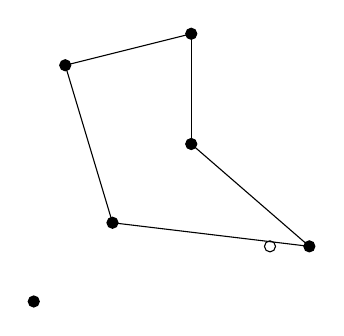
\begin{tikzpicture}
\draw[fill] (0,0) circle (2pt) coordinate (a);
\draw[fill] (0.4,3) circle (2pt) coordinate (b);
\draw[fill] (2,3.4) circle (2pt) coordinate (c);
\draw[fill] (3.5,0.7) circle (2pt) coordinate (d);
\draw[fill] (1,1) circle (2pt) coordinate (e);
\draw[fill] (2,2) circle (2pt) coordinate (f);
\draw[] (3,0.7) circle (2pt) coordinate (g);
\draw (b)--(e);
\draw (e)--(d);
\draw (b)--(c);
\draw (c)--(f);
\draw (f)--(d);
\end{tikzpicture}}
\caption{Intermediate addition.}
\label{subfig:increasing_loop_step_3}
\end{subfigure}
\begin{subfigure}{0.3\textwidth}
\centering
\fbox{\begin{tikzpicture}
\draw[] (0,0) circle (2pt) coordinate (a);
\draw[fill] (0.4,3) circle (2pt) coordinate (b);
\draw[fill] (2,3.4) circle (2pt) coordinate (c);
\draw[fill] (3.5,0.7) circle (2pt) coordinate (d);
\draw[fill] (1,1) circle (2pt) coordinate (e);
\draw[fill] (2,2) circle (2pt) coordinate (f);
\draw[fill] (3,0.7) circle (2pt) coordinate (g);
\draw (b)--(e);
\draw (b)--(c);
\draw (c)--(f);
\draw (f)--(d);
\draw (g)--(d);
\draw (g)--(e);
\end{tikzpicture}}
\caption{Final addition.}
\label{subfig:increasing_loop_step_4}
\end{subfigure}
\begin{subfigure}{0.3\textwidth}
\centering
\fbox{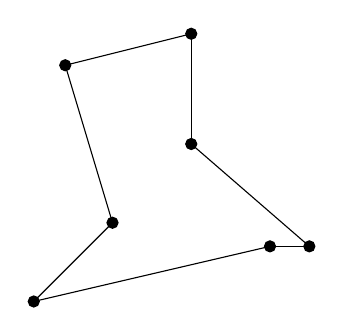
\begin{tikzpicture}
\draw[fill] (0,0) circle (2pt) coordinate (a);
\draw[fill] (0.4,3) circle (2pt) coordinate (b);
\draw[fill] (2,3.4) circle (2pt) coordinate (c);
\draw[fill] (3.5,0.7) circle (2pt) coordinate (d);
\draw[fill] (1,1) circle (2pt) coordinate (e);
\draw[fill] (2,2) circle (2pt) coordinate (f);
\draw[fill] (3,0.7) circle (2pt) coordinate (g);
\draw (b)--(e);
\draw (b)--(c);
\draw (c)--(f);
\draw (f)--(d);
\draw (g)--(d);
\draw (g)--(a);
\draw (e)--(a);
\end{tikzpicture}}
\caption{Final route.}
\label{subfig:increasing_loop_step_5}
\end{subfigure}
\caption{Progression of the increasing loop algorithm. Empty circles  represent the next global minimum for the next iteration.}
\label{fig:increasing_loop}
\end{figure}

\subsubsection{\texttt{forcefully\_increasing\_loop}}
\label{subsubsec:forcefully_increasing_loops}

\begin{flushright}
\textbf{Author} \\
Oliver Sheridan-Methven
\end{flushright}

This algorithm is a quicker and less exhaustive implementation of the increasing loop algorithm as described in Section~\ref{subsec:increasing_loop}

The algorithm begins by randomly selecting three vertices and forming a loop between them, containing only these three\footnote{We can assume that we have more than 3 vertices, else the solution is trivial.}. Then with this sub-loop, we consider random vertex not contained in the sub-loop. For this unconnected vertex, we evaluate the added distance to the loop if we were to include this vertex and form a larger sub-loop. We compute which connection in the loop would need to be changed that would given the minimal distance increase. We increase the sub-loop using this vertex to the configuration just previously computed. We perform this scheme iteratively until there are no unconnected vertices. A depiction of the scheme is shown in Figure~\ref{fig:increasing_loop}.



